\chapter{The Flatland Model}
In order to become good at picking locks, you will need a detailed understanding of how locks works and what happens as it is picked.
This document uses two models to help you understand the behavior of locks.
This chapter presents a model that highlights interactions between pin positions.
Chapter 4 uses this model to explain how picking works.
Chapter 9 will use this model to explain complicated mechanical defects.

The "flatland" model of a lock is shown in Figure 3.1. This is not a cross section of a real lock.
It is a cross section of a very simple kind of lock.
The purpose of this lock is to keep two plates of metal from sliding over each other unless the proper key is present.
The lock is constructed by placing the two plates over each other and drilling holes which pass through both plates.
The figure shows a two hole lock. Two pins are placed in each hole such that the gap between the pins does not line up with the gap between the plates.
The bottom pin is called the \textit{key pin} because it touches the key.
The top pin is called the \textit{driver pin}. Often the driver and key pins are just called the driver and the pin.
A protrusion on the underside of the bottom plate keeps the pins from falling out, and a spring above the top plate pushes down on the driver pin.

If the key is absent, the plates cannot slide over each other because the driver pins pass through both plates.
The correct key lifts the pin pairs to align the gap between the pins with the gap between the plates.
See Figure 3.3. That is, the key lifts the key pin until its top reaches the lock's sheer line.
In this configuration, the plates can slide past each other.

Figure 3.3 also illustrates one of the important features of real locks.
There is always a sliding allowance.
That is, any parts which slide past each other must be separated by a gap.
The gap between the top and bottom plates allows a range of keys to open the lock.
Notice that the right key pin in Figure 3.3 is not raised as high as the left pin, yet the lock will still open.

\begin{figure}
    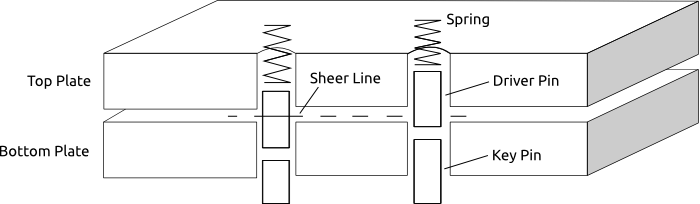
\includegraphics[width=\textwidth]{figure3.1}
    \caption{Flatland model of a lock}
\end{figure}

\begin{figure}
    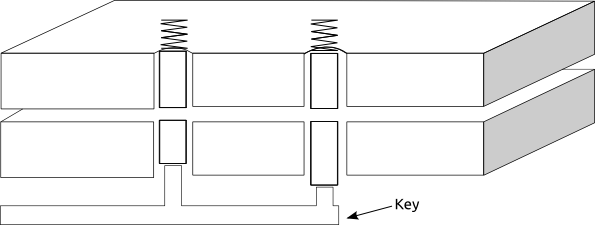
\includegraphics[width=\textwidth]{figure3.2}
    \caption{(a) Flatland key raises pins}
\end{figure}

\begin{figure}
    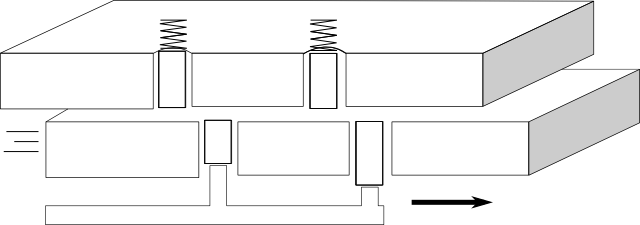
\includegraphics[width=\textwidth]{figure3.3}
    \caption{(b) Proper key allows plates to slide}
\end{figure}